\chapter{Motivation}
\label{ch:motivation}

\newthought{In 1905, William Bateson, Edith Saunders, and Reginald Punnett} published results on their work with dihybrid crosses of pea plants.  Having previously established the dominance of two phenotypes (purple flowers over red, and long pollen grains over round), the trio crossed pea plants exhibiting both dominant or both recessive traits for successive generations.  Crossing the first generation was expected to yield progeny with phenotype ratios following the $9$:$3$:$3$:$1$ pattern according to the Law of Independent Assortment, established by Gregor Mendel $40$ years prior.  However, the observed ratios differed wildly from this expectation, heavily skewed towards the parental combination of phenotypes.  Bateson \textit{et al.} hypothesized that alleles controlling the two traits must be linked and transmitted to the progeny together by some unknown mechanism~\cite{Bateson:1908dq}.

Seven years later, Thomas Morgan noted an even more aberrant inheritance pattern in a dihybrid cross of white-eyed male and red-eyed female \textit{Drosophila melanogaster} flies: no white-eyed females were observed in the progeny.  A follow-up experiment crossing the original white-eyed male with its $F_{1}$ daughters produced four roughly equal-sized groups of red-eyed and white-eyed males and females, suggesting the white-eyed factor must be linked to the male sex factor.  Morgan proposed that these factors (what we now refer to as genes) are real entities, physically located on chromosomes, and when found on the same chromosome, do not (necessarily) sort independently~\cite{Morgan:1910hg}.

Today, linkage analysis in experimentally controlled crosses (like the pea plants and fruit flies) or pedigrees (multi-generational families) is an invaluable tool in the study of genetics.  Progeny only inherit half of their genome from each parent, so having several progeny that still exhibit the parental phenotypes helps narrow the region of the genome one must search to find the relevant genes.  Modern experiments exploit the recombinant nature of genomes to unravel myriad phenotypes, the genes that control them, and the underlying genome biology responsible.  These approaches have been broadly applied, proving particularly valuable in pathogens.  For example, crosses of \textit{Plasmodium falciparum} parasites, the causative agent for the most deadly form of malaria, have led to the discovery of a number of virulence factors.  Several contrasting phenotypes for various strains of \textit{P. falciparum} are listed in Table \ref{tb:pf_phenotypes}.  Crossing of the pyrimethamine-resistant 3D7 and sensitive HB3 strains~\cite{Walliker:1987cv} revealed a nonsynoymous point mutation in the \textit{dhfr-ts}\footnote{dihydrofolate reductase-thymidylate synthase} gene, inhibiting binding of (and thus conferring resistance to) the drug~\cite{Peterson:1988wt}.  Analysis of the HB3 x DD2 cross\cite{Wellems:1990eg}, the latter of which is resistant to chloroquine, localized the determinant to a previously undetected gene on chromosome $7$, labelled \textit{pfcrt}\footnote{\textit{P. falciparum} chloroquine resistance transporter}, a member of a new family of transporters.  Additional investigation into differences in mosquito infection efficacy revealed down-regulation of the \textit{pfmdv-1}\footnote{\textit{P. falciparum} male gametocyte development gene 1} gene~\cite{Vaidya:1995up,Furuya:2005jn}, disruption of which results in marked reduction of mature and functional male gametocytes.

\begin{table}[]
\centering
\caption{Phenotypes of \textit{P. falciparum} isolates used for genetic crosses.}
\label{tb:pf_phenotypes}
\begin{tabular}{@{}rcccccc@{}}
\toprule
                                 & 3D7 & HB3 & DD2 & 7G8 & GB4 & 803 \\
\midrule
pyrimethamine sensitivity        & -   & +   &     &     &     &     \\
chloroquine sensitivity          &     & +   & -   &     &     &     \\
infects mosquitoes easily        &     & +   & -   &     &     &     \\
infects \textit{Aotus nancymaae} &     &     &     & -   & +   &     \\
\bottomrule
\end{tabular}
\end{table}

Many clinically relevant phenotypes are not inherited, but instead arise anew within the children.  Cytoadherence and antigenic properties of parasites facilitate evasion from host immune attack, and can differ substantially from the properties of their progenitors.  In 2000, Freitas-Junior \textit{et al.} showed that some 3D7 x HB3, HB3 x DD2, and HB3 x HB3 progeny harbored non-parental forms of subtelomeric \textit{var} genes, key members of an antigenic gene family\cite{FreitasJunior:2000cp}.  These altered forms were likely generated during mitosis by non-allelic homologous recombination\footnote{sometimes referred to as "ectopic" (aberrant) recombination in the literature} (NAHR) of telomeres from two different chromosomes\cite{Duffy:2009cc}.  The resulting genes are novel, functional, and never before observed by the host immune system.

These uninherited and spontaneous, or "\textit{de novo}" mutations (DNMs) are critical tools for pathogenic adaption (and perhaps in higher-order organisms, maladaption).  Pathogens are under constant immune and intermittent drug pressure.  NAHR serves to further diversify a pathogen's antigenic repertoire, enabling continued evasion of immunological actors.  Random, spontaneous point mutations eventually produce a drug-resistant parasite, capable of surviving the onslaught and reproducing.

With the advent of sequencing technologies, it is now straightforward to discover many DNMs.  Long reads (\textasciitilde $500$ bp) from the first-generation sequencing technology, Sanger sequencing, can be stitched together \textit{in silico} by considering the overlaps of sequences generated from many copies of the genome\cite{Myers:1995vma}.  This has enabled the assembly of full-length genomes and subsequent gene annotations for a single representative (or "reference") individual in a population.  Second-generation sequencing is leveraging economies of scale to reduce sequencing costs by several orders of magnitude\cite{Mardis:2011cr}.  The reads it produces are shorter (\textasciitilde $100$ bp) and more error-prone, but billions of them can be produced quickly.  Like the long reads, the short read data can also be assembled into a new genome, albeit with more errors and gaps, owing to the difficulty of overcoming large repetitive regions with short genomic fragments\cite{Schatz:2010if}.  Alternatively, assuming the sequence for the reference genome and a new individual are highly similar, it is far more common (and computationally more efficient) to align the reads to the reference\cite{Flicek:2009dl}.  String matching algorithms that allow mismatches, insertion, and deletions to appear in the alignments allow millions of sequnced reads to be placed on the reference genome quickly.  Separate tools can then examine the alignments, looking for the presence of non-reference alleles, and using statistical approaches to call and genotype variants with high accuracy\cite{Nielsen:2011kz}.

Variant calling software has been successfully applied to many sequencing datasets for the discovery of DNMs.  These variant callsets have provided insight into the development of drug resistance\cite{Woodford:2007it}, the genetic architecture of some common diseases\cite{Neale:2012ki}, and mutational rates in humans and chimpanzees with a strong paternal age effect.\cite{Conrad:2011eh,Venn:2014ep,Kloosterman:2015cn,Francioli:2015kj}.  Many groups have released sophisticated software packages to facilitate these analyses and detailed instructions on their use\cite{DePristo:2011fo,Rimmer:2014ho}.

Specificity and sensitivity are crucial metrics to consider for any variant callset.  There are many approaches to establishing the specificity of a DNM callset.  For select variants (typically on the order of \textasciitilde $100$ variants from a callset), Sanger sequencing, Sequenom assays, and even targeted third-generation sequencing (i.e. PacBio sequencing, which can generate reads up to \textasciitilde $50,000$ bp as of this writing) have been used successfully to validate mutations.  Establishing sensitivity is much more difficult, and in some cases, overall sensitivity to DNMs will be much lower than one might initially appreciate.  The underlying assumption that two genomes from the same species should be very similar is likely inappropriate for highly diverse populations (e.g. pathogens) or hypervariable regions (e.g. immune loci in mammals).  If a haplotype present in the sample is too dissimilar to the reference, or perhaps even completely absent, read aligners may return incorrect results.  Reads may align to the wrong location, the resultant mismatches mistaken for real mutations.  Alternatively, they may fail to align at all, thus obscuring evidence of real variation.

Instead, it may be possible to establish the sensitivity of the reference-based protocol by considering how DNMs alter the genome of a sample with respect to its progenitors.  Consider a site where a DNM - say, a single SNP - has occurred, as depicted in Figure \ref{fig:kmer_venn}.  Although a single base of the genome has been altered, when the genome is divided into fixed-length words of length $k$, or "kmers", we find $k$ kmers that are present in the child but absent in the parents.  In this manner, DNM could be considered generators of "novel" kmers.  These kmers can be used as a signal to indicate the presence of a \textit{de novo} variant.  By choosing $k$ to be reasonably large so as to avoid analyzing short sequences that pervade the genome (half to two-thirds the length of a read will suffice), we can simply count continuous stretches of novel kmers as a proxy for the number of DNMs.

\begin{figure}[h!]
  \centering
    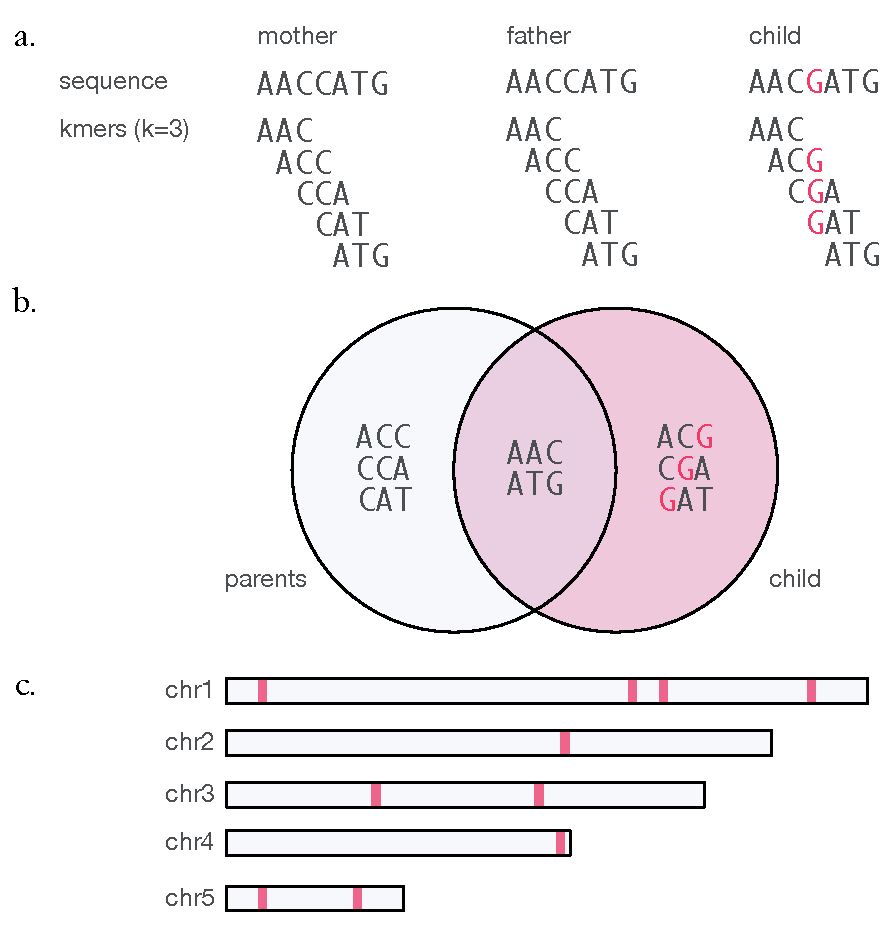
\includegraphics[width=\textwidth]{kmer_venn}
  \caption{a. Parental and child sequences at the site of a \textit{de novo} mutation, and the kmers generated at $k=3$.  b. The resulting Venn diagram of kmers found exclusively in the parents, the child, or common to both.}
  \label{fig:kmer_venn}
\end{figure}

Similarly, if we regard DNM to be generators of novelty, the de novo variant calls we produce with the reference-based protocol should yield an identical set of novel kmers.  One must simply take all of the variant calls (inherited and de novo events) obtained for the child and apply this as a delta to the reference genome.  At de novo mutations, we extract the local sequence context and divide the data into kmers.  If the reference-based analysis and reference-free analysis yield similar number of kmers, then we have found all of the de novo variants.

